\documentclass[a4paper]{jarticle}
\usepackage{tani_resume}
\usepackage{epstopdf}
\usepackage{graphicx}
\usepackage{ascmac}
\alignbeforeskip -5mm
\alignafterskip -5mm
\eqnarraybeforeskip -5mm
\eqnarrayafterskip -5mm
\makeatletter
\newenvironment{figurehere}
  {\def\@captype{figure}}
  {}
\makeatother

\jptitle{France-IOI提供の国際情報科学コンテストBebras Challenge用コンテスト環境bebras-platformの試運用}
\etitle{}
\jpauthor{鈴木一至 佐々木陽広}
\eauthor{Kazushi Suzuki,Akihiro Sasaki}
\course{谷聖一研究室}
\year{27}


%% 概要 %%
\abstract{
コンピュータ・サイエンスの普及を目的とした取り組みは,様々なところで行われている.
その中の1つに,小・中・高校生を対象にした「Bebras Challenge」がある.Bebras Challengeは,情報科学に触れてもらうことを目的とし,情報科学の事前知識がなくても解くことが可能なオンラインコンテストである.Association France-IOIがBebras Challenge開催用のサーバシステムである「bebras-platform」を開発し,オープンソースとして公開している.bebras-platformには,コンテストを開催するだけでなく,過去に行ったコンテストへ挑戦できる機能もある.本演習では,bebras-platformを利用して,日本でのコンテストサーバ運用のノウハウ蓄積と,過去に実施されたBebras Challengeの問題へ挑戦できる環境を構築した.}
\compheading

\begin{document}
\maketitle
\begin{multicols}{2}
\setcounter{page}{1}

\section{はじめに}

\subsection{Bebras Challenge}
\subsubsection{Bebras Chalengeの概要}
Bebras Challenge(\cite{bebras-contest, bebras-pdf})とは,2004年にリトアニアで始められた国際的な情報科学コンテストである.日本では,年に1回開催され,小学5年生から高等学校3年生を対象としている.日本は2011年度から正式参加しており,2015年には世界35カ国から130万人の児童・生徒が参加している.情報科学の事前知識がなくても解くことが可能な問題を扱い,問題に取り組むことによって情報科学の基礎概念に触れることができ,論理的思考の向上の一助になるようなものになっている.また,コンテスト後に参加者同士で問題の内容について議論することで,情報科学に興味を持つきっかけになることが期待される.

\subsubsection{Bebras Challengeの形式}
 コンテストはオンラインで開催され,参加者はブラウザなどを通して参加する.コンテストの問題は年齢に応じた区分ごとに用意されており,基本はベンジャミン(小学5年生・6年生),カデット(中学1年生・2年生),ジュニア(中学3年生・高校1年生),シニア(高校2年生・3年生)の4区分であり,日本ではベンジャミンが30分10問,その他が40分12問で実地している.
\\ 問題形式は大きく2種類あり,動的にオブジェクトを操作しながら試行錯誤できる対話型と,それに対する非対話型がある.また,非対話型の中には選択肢を選んで解く選択肢型と,文字を入力して解答する文字入力型がある.

\subsection{国際情報オリンピック}
国際情報オリンピック(International Olympiad in Informatics, IOI)(\cite{ioi})とは,1989年から毎年行われる高校生を対象としたプログラミング能力を競う国際大会である.高校生以上を対象とし,その能力の育成を助け,各国の選手・教育者同士の国際交流を図ることを目的をする.
\subsection{情報オリンピック日本委員会}
日本では,国際情報オリンピックに日本代表選手を派遣するために,情報オリンピック日本委員会が日本情報オリンピックを主催している.(詳細は\cite{joi}参照)
\\ 中には,数理情報科学の復旧・啓発のために,主に小中学生向けのイベントの開催やウェブコンテンツの開発・公表を行っている情報オリンピック日本委員会ジュニア部会がある.Bebras Challengeは,この日本委員会ジュニア部会によって参加推進等の活動が行われている.


\subsection{Association France-IOI}
Association France-IOIは,国際情報オリンピックのフランスチームの選出と育成を目的とし2004年に設立された.フランスでのBebras Challengeを主催しており,Bebras Challenge開催用のサーバシステムであるbebras-platformをオープンソースとして公開している.
\\ Association France-IOIは,2011年からBebras Challengeを主催しており,2015年には世界各国で最も多い35万人もが参加する規模になっている.
\subsection{演習目的}
Bebras Challengeを実施するためには,コンテスト環境を提供するサーバシステムが必要であるが,リトアニア,オランダ,フィンランド,台湾,フランスはサーバシステムを開発し運用している.日本ではオランダのサーバを利用しBebras Challengeを開催しているが,コンテストに参加する教育機関のコンテンツフィルターやファイヤーウォール機器の性能も含めたネットワーク環境によっては正常にコンテストに参加することが困難な場合があった.
\\ この問題を緩和する方法の1つとして,ネットワーク的に近いコンテストサーバを運用するという手段が挙げられる.Association France-IOIによるオープンソースのサーバシステムであるbebras-platformを利用することで,正常にコンテストに参加できない教育機関の減少を期待できると考えた.本演習の目的は,このbebras-platformを用いてBebras Challengeのサーバを運用するためのノウハウの蓄積と,事後学習のための過去に実施されたコンテストへの挑戦を可能にすることである.

\section{bebras-platform}


\subsection{構成}
bebras-platformは,サーバ全体ではなくHTMLやPHPなどのファイルやデータベースを構成する要素の集合体である.サーバ環境を構築する上では,httpdとして「Apache」,データベースマネージメントシステムとして「MySQL」を利用することが前提とされている.しかしサーバ環境のOSには縛りはなく,開発者のニーズに合ったOSを選択することが可能となる.また,bebras-platformはオープンソースソフトウェアであるため,随時変更・改変が行われる.
%Webサーバソフトウェア(Apache)とデータベース管理システム(MySQL)の変更できないが,実装する環境のOSに縛りはなく,開発者のニーズに合ったOSを選択することが可能になっている.また,このbebras-platformは更新が行われるので,随時適応する必要がある.

\subsection{使用ツール}
\begin{description}
\item[Git]プログラムのソースコードなどの変更履歴を記録・追跡するための分散型バージョン管理システムである.また,Gitを使用してソフトウェア開発プロジェクトのための共有ウェブサービスとしてGithubがある.(詳細は\cite{git}参照)\\ bebras-platformは,Github上で公開されており,随時更新が行われている.
\end{description}

\begin{description}
\item[Bower]Twitter社によるフロントエンド用パッケージ管理ツールである.JSON形式の設定ファイルを用意することで,記述されたパッケージを一括で取り込むことができる.(詳細は\cite{bower}参照)
\end{description}

\begin{description}
\item[Composer] PHPの依存関係管理ツールである.Bowerと同様にJSONファイルから複数のパッケージのインストールが可能である.(詳細は\cite{composer}参照)
\end{description}

\begin{description}
\item[DBV]  Webページ上でデータベース管理を行うためのツールである.主にAssociation France-IOIのプロジェクトに使用される.(詳細は\cite{dbv}参照)
\end{description}

\begin{description}
\item[i18next] フロントエンドにて国際化を可能にするライブラリである.JSONと呼ばれるデータ記述形式に対応する訳記入することで,対応する単語を翻訳することが可能である.(詳細は\cite{i18n}参照)\\bebras-platformのHTML上では,data-i18n属性を用い,それぞれ翻訳箇所に任意の文字列を入力し使用する.
\end{description}

\subsection{ページ構造}
bebras-platformのユーザ用のページは2種類存在する.1つ目はコンテスト参加者が利用するページである(図\ref{fig:1}参照).コンテストの参加や過去問の参照を行うことができる.
\begin{figurehere}
\begin{center}
\fbox{
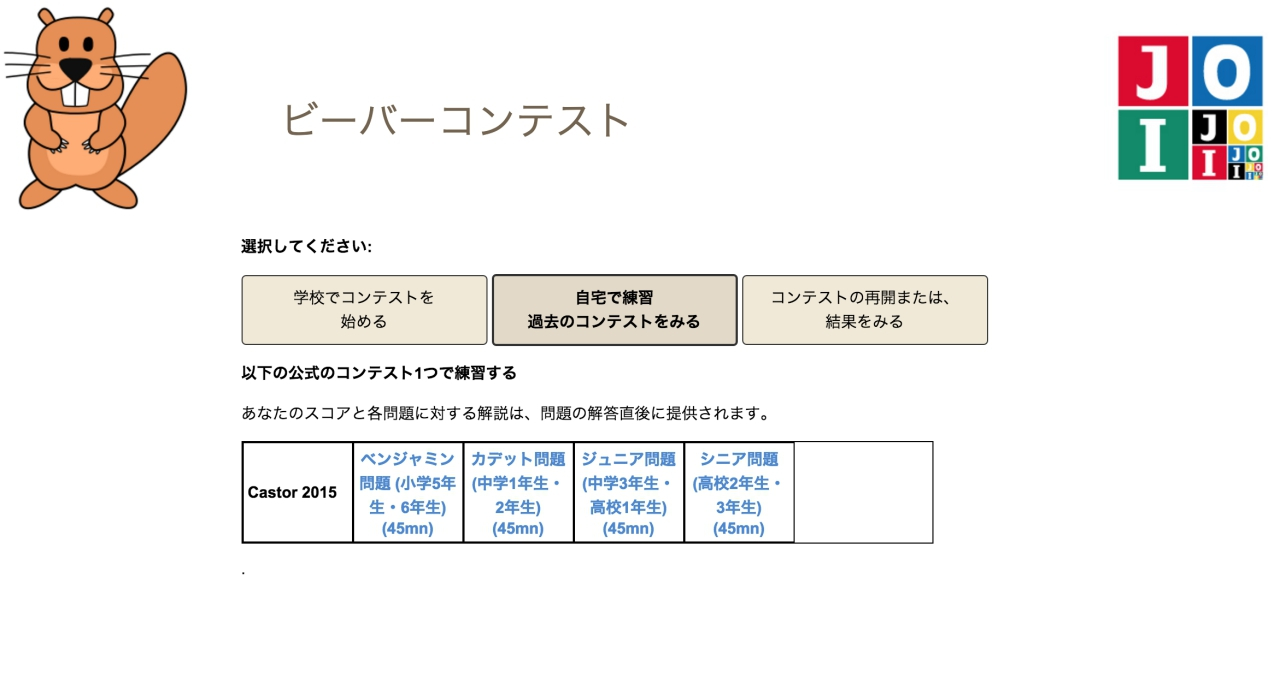
\includegraphics[bb=0 0 1280 679,width=8cm]{img/bebras_top.jpg}
}
\end{center}
\caption{bebras-platformの参加者用ページ}\label{fig:1}
\end{figurehere}

2つ目は管理者が利用するページである(図\ref{fig:2}参照).コンテスト(サイト)の管理者がログインし,コンテストの作成や問題の追加を行うことができる.

\begin{figurehere}
\begin{center}
\fbox{
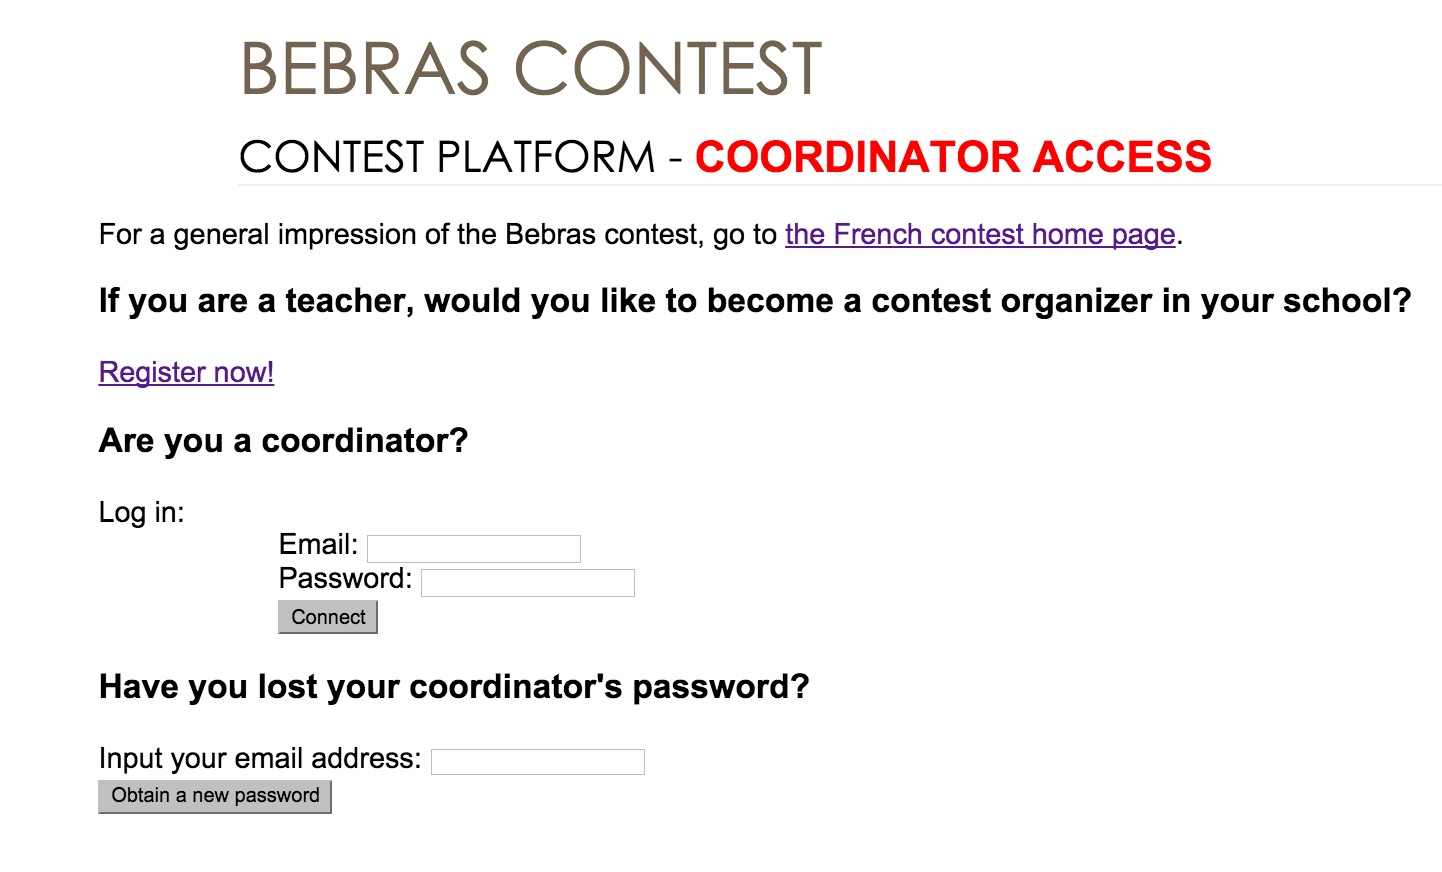
\includegraphics[bb=0 0 1442 872,width=8cm]{img/admin_top.jpg}
}
\end{center}
\caption{bebras-platformの管理者用ページ}\label{fig:2}
\end{figurehere}



\subsection{ユーザ}
\begin{description}
\item[管理者]  ユーザの中で最も強い権限を持ち,問題(タスク)の追加,コンテストの作成や自分以外のユーザの認証が可能である.ただし最初の管理者の登録はデータベースを直接変更する必要がある. 
\end{description}

\begin{description}
\item[教師] 管理者の下位互換的な役割であり,問題やコンテストの作成はできないが,コンテストの行うためのグループの作成が可能なユーザである.教師はユーザ登録後に管理者に認証してもらう必要がある.
\end{description}

\begin{description}
\item[参加者] 管理者,教師以外のユーザとして参加者がある.参加者は,コンテストの参加,過去問の参照が可能となっており,コンテスト参加時に発行されるグループコードを入力することで,コンテストの結果を参照することも可能である.
\end{description}




\section{bebras-platformの試運用}
\subsection{コンテスト環境の構築}
\subsubsection{翻訳}
bebras-platformのインターフェイスは大部分が英語であり,また一部はフランス語で記述されている.コンテスト参加者がスムーズにコンテストを受けるためには,インターフェイスの日本語化が必要不可欠であった.そこでi18nextを利用し翻訳を行った.しかし,一部のコード内に文字が埋め込まれている箇所の翻訳はi18nextで対応することは不可能であったため,その箇所の翻訳は直接コードの変更を行い対応した.
\subsubsection{過去問の追加}
2014,2015年度の過去のコンテスト問題を過去問として公開した.問題はbebras-platformのサンプル問題を参考にテンプレートを作成し,そのテンプレートを編集する形で問題を追加した.本演習では,
%一部機能の実装となっているため,
非対話型の問題形式のみ追加を行った.

\subsection{開発管理環境}
bebras-platformを公開するまでの流れとして様々な手段があるが,随時Githubにて更新されるため,運用手順を明確化する必要があった.本演習では,一度手元の環境でサーバシステムを構築し,ローカル環境をそのまま本番環境へコピーする形で運用している.このようにすることでBowerなどの管理系ツールを本番環境へ導入する必要がなくなり,更にローカル環境で一度実装することによって本番環境での不具合によるリスクを減らすことが可能である.

\subsection{ドキュメント作成}
bebras-platformはAssociation France-IOI提供のシステムであるため,日本語での記載は一切なく,実装に至るまで様々な試行錯誤を経た.報告者は,蓄積したノウハウの共有のためドキュメントの作成を行った.このドキュメントは環境構築手順から現在の運用状況など報告者以外の人がこの試運用したbebras-platformを手間なく理解するための仕様書である.元のbebras-platformは随時更新されるため,必要に応じてこのドキュメントも整理することが今後重要である.

\section{終わりに}
本演習では,Association France-IOIによるbebras-platformを利用して,Bebras Challenge用コンテスト環境を構築した.
\\ 追加した過去のコンテスト問題は非対話型の形式のみの対応となっているため,対話型問題の実装が今後の課題となる.また,問題を作成するにあたってテンプレートは作成したが,問題の選択肢,解答などの要素をそれぞれ手動で入力する必要があるため,この問題作成までの一連の流れの自動化が,改善点の1つとして挙げられる.
\\ bebras-platformを利用し,過去のコンテスト問題だけでなく,実際のBebras Challengeの開催も視野入れていたが,bebras-platformの実装と時期が合わず,2015年度での開催はできなかった.そのため2016年度以降のBebras Challengeの開催も今後の課題となる.

\end{multicols}

%%%%% 参考文献 %%%%%
\begin{thebibliography}{1}

\bibitem{bebras-contest} 「ビーバーコンテスト」情報ページ.  http://bebras.eplang.jp/ , (参照 2015-12-08)
\bibitem{bebras-pdf} 谷 聖一, 兼宗 進, 井戸坂 幸男. 小中高生向け国際情報科学コンテストBebras.  http://www.ipsj.or.jp/magazine/9faeag0000005al5-att/peta55-11.pdf, (参照 2015-12-08)
\bibitem{bebras-france-platform} Bebras Platform. https://github.com/France-ioi/bebras-platform
\bibitem{ioi} 国際情報オリンピック http://www.ioinformatics.org/index.shtml   http://www.ioi-jp.org/ioi/
\bibitem{joi}日本情報オリンピック委員会 https://www.ioi-jp.org/
\bibitem{git} Git  https://ja.wikipedia.org/wiki/Git
\bibitem{bower}Bower  http://bower.io/
\bibitem{composer}Composer  https://getcomposer.org/
\bibitem{dbv}dbv  http://dbv.vizuina.com/
\bibitem{i18n}i18n  http://i18next.com/



\end{thebibliography}

\end{document} 




